
When you are in a situation you haven't been in before, a guidebook can decrease anxiety by making the unfamiliar less intimidating. 
A guidebook labels patterns and provides context for your observations. 
Recognizing a familiar challenge can be preferable to the uncertainty of facing a scenario that is novel. A situation that is unfamiliar means not knowing how to start and what the potential paths to success are. In contrast, a challenge that is understood from the start can feel less burdensome. Even a challenge that is understood requires creativity and effort.

Bureaucracy is a consistent and pervasive challenge in modern society. You probably have direct experience with bureaucracy, and you may be familiar with complaints about bureaucracy. You probably don't consider yourself a bureaucrat, and probably are not an expert on bureaucracy.

%If you don't think of yourself as a bureaucrat, I hope to change your mind on this essential topic. 

Negative impressions of bureaucracy are common. The word
%bureaucracy 
% 2022-07-09: Jonah@upwork advocates removing this use
evokes reactions of disgust, primarily driven by how individuals have experienced bureaucracy.
The results of bureaucracy can appear idiotic.
Bureaucracy is even regarded as dangerous to society\footnote{``The only thing that saves us from the bureaucracy is inefficiency. An efficient bureaucracy is the greatest threat to liberty." -Eugene McCarthy (1979)}.
I have bad news for you if you have a negative impression of bureaucracy: bureaucracy is vital to society. 
% Effective bureaucracy is  to modern society.
Organizations have an insatiable need for members to perform a variety of tasks.

The good news is that you can learn to skillfully navigate bureaucracy. The consequence is that a skilled bureaucrat is more effective. That improvement enhances the organization you are part of. Modern society is an interwoven fabric of organizations, with  bureaucracy being the crucial material.
Rather than ponder societal-scale concerns, the focus of this book is on the complex and typical experience of a bureaucrat. 


The framing of how you think about bureaucracy shapes what action you think is relevant for changing your environment. 
If your assumptions are wrong about how the system of bureaucracy works, then you will be trying to convert the system to meet your incorrect expectations and your actions are likely to be wasted effort tackling irrelevant aspects. 
An accurate model of bureaucracy allows you to be more effective and your changes to the system are more likely to succeed. 

Having a precise definition of bureaucracy enables a clearer discussion. 
\begin{quote}
\textbf{Definition}: \Gls{bureaucracy} is the management of shared resources, whether tangible or expertise, by subjective decision making of individual people using distributed knowledge and distributed decision making. 
\end{quote}

The concepts and techniques in this book are derived from this definition. For more exploration of this definition, see the section ``\hyperref[sec:define-bureaucracy]{What is Bureaucracy?}'' on page~\pageref{sec:define-bureaucracy}.

As an example of how the above definition is distinct from conventional definitions\footnote{\href{https://www.merriam-webster.com/dictionary/bureaucracy}{Merriam-Webster's definition} focuses on government; the \href{https://www.merriam-webster.com/dictionary/bureaucracy}{Wikipedia entry} acknowledges non-governmental bureaucracy.}, I view government as an instance of where bureaucracy occurs. Bureaucracy is not limited to government. I use the term ``organization'' to encompass governments, corporations, non-profits, or any collection of people working together. As a consequence, a vast majority of people are bureaucrats. 

The negative connotation of bureaucracy may lead you to reject the label of bureaucrat. Your recognition of your status as a bureaucrat matters even if you intentionally reject the label or simply do not recognize that you are bureaucrat, self-. How you behave and what you think your responsibilities are depend on how you label yourself.
% If you do not recognize that you are bureaucrat, you're less likely to be successful interacting with those around you. 
If you don't think of yourself as a bureaucrat, then you won't be able to distinguish what is your own fault, what is the fault of your coworkers, what is the fault of management, and what is intrinsic to bureaucracy. 

Reasoning about bureaucracy is an accessible topic for every reader because we each have personal experience.
A commonly held view is that the systems of bureaucracy that we work within are broken: participants are harmed and there is inequality. 
The counterargument is that the bureaucratic behavior observed is how the system was designed to work. There is a third argument: bureaucratic systems work in a degraded mode -- being less efficient than what is possible. 
In this book I set aside the macro-scale questions of bureaucracy like the three arguments above and focus on the human-scale interactions that give rise to bureaucracy.

Even people who are smart (e.g., they know history, they have memorized capital cities, they can do math) can struggle when faced with complex large-scale distributed systems comprised of humans. Thinking about complex large-scale systems is not part of the conventional education curriculum. This book will help you learn about bureaucracy, increase your ability to identify patterns, and apply relevant techniques.


The difficulties of bureaucracy are central to large societies that depend on complex interactions of many people. The challenge of bureaucracy is widespread across a variety of governments and companies in different societies. And bureaucracy is durable -- it has existed for thousands of years. Because bureaucracy is pervasive, tackling the topic of bureaucracy is exciting and crucial. The excitement comes from the opportunities available for the many potential improvements.
%I enjoy pondering hard problems and then leveraging insights gained from reflection.
Being an effective bureaucrat is important because bureaucracy can be a \href{https://en.wikipedia.org/wiki/Force_multiplication}{force multiplier} beyond what one person could accomplish on their own.

% Who this book is for

% from https://graphthinking.blogspot.com/2021/07/bureaucracy-book-outline.html
This book is for you if you are curious about the complex world we live in, or if you are thinking about how to productively contribute to society, or if you want impactful employment, or if your job is not what you expected. If you're wondering why innovation is hard within a bureaucratic organization, this guidebook is intended to help you understand the challenges. Understanding the challenges means you can design ideas that are more likely to succeed.


% What you should expect reading this book: 
Every person in society is a participant in bureaucracy. The purpose of this book is to decrease the surprise of that experience and better prepare you emotionally and intellectually for the toil of being a bureaucrat. With focused reflection and a good guidebook, you can improve your skills as a bureaucrat. 

Understanding bureaucracy spans academic disciplines - \href{https://en.wikipedia.org/wiki/Psychology}{psychology}, \href{https://en.wikipedia.org/wiki/Sociology}{sociology}, \href{https://en.wikipedia.org/wiki/Organizational_behavior}{organizational dynamics}, \href{https://en.wikipedia.org/wiki/Public_administration}{public administration}, \href{https://en.wikipedia.org/wiki/Anthropology}{anthropology}, and  \href{https://en.wikipedia.org/wiki/Political_science}{political science}. Most bureaucrats have no formal training in any of these domains. This book is not written from the academic perspective; it is written by a practicing bureaucrat to serve as a guidebook to be read by bureaucrats. 

This book is not a defense of bureaucracy, nor is it intended to disparage bureaucrats or the system of bureaucracy. Instead, the intent of this book is to serve as a guide to bureaucracy-as-it-is. There are no hacks presented for circumventing bureaucracy. Instead, this book provides advice on being an effective member of a bureaucratic organization.

This book does not focus on leadership, managing a team, being a team member, planning, time management, project management, advancing your career, promotions, or self-improvement. In the process of being a better bureaucrat some lessons may apply in those domains.


Nothing in this book is domain specific, nothing is tied to engineering of products, and nothing is applicable solely in science research or policy development. However, the skills associated with being an effective bureaucrat do translate into other domains.

This book doesn't address personal stress caused by bureaucracy, how to decrease stress, or how to balance the activities of work and life-outside-work.   However, understanding bureaucracy can enable a positive sense of self based on how your efforts integrate with other people's tasks. 

This book does not address work conditions, pay, benefits, or retirement plans. If you are seeking a competitive advantage that might result in improved outcomes, learning how to navigate bureaucracy helps.


This book doesn't focus on citizens, political policy makers, oversight (e.g., Congress -- state or federal), competing organizations, contracts, the budget of an organization, fines and other regulatory punishments resulting from bureaucracy, policy enforcement, specific policies and regulations, formal arbitration or judicial resolution of disputes. For observations on those topics, see Wilson's Bureaucracy~\cite{1991_Wilson}. 


This book doesn't address discrimination or harassment. I neglect differences of experience based on the race, gender, or socioeconomic status. This book doesn't address bad coworkers, abusive bosses, psychological defects of individuals, or malicious intent. I assume no traitors, spies, or \href{https://www.hsdl.org/?abstract&did=750070}{saboteurs}\footnote{See also Wikipedia's entry for the \href{https://en.wikisource.org/wiki/Simple_Sabotage_Field_Manual}{Simple Sabotage Field Manual}}.
I do not address \href{https://en.wikipedia.org/wiki/Dark_pattern}{dark patterns}; issues like lying, bribery~\cite{2021_Ang}, and criminal behavior are not discussed. All these aspects happen whenever people interact; those challenges are not specific to bureaucracy. 
Bureaucracy is not a manifestation of incompetence, malicious actors, or mistakes. The source of friction in a well-run bureaucracy is human interactions and ambiguity.


In this book I assume you are honest, and that other people are honest.  
I assume bureaucrats strive for fairness, though the particular definition of fairness may vary from bureaucrat to bureaucrat. 
Even with all these simplifying assumptions the complexities of bureaucracy arise. My guidance on how to be an effective bureaucrat is in the context of benign bureaucracy.


% What is the benefit of reading this book?
As a result of reading this book, you will be better able to recognize and navigate complex professional environments, both within your career and outside of work. Perspectives offered in this book can benefit you directly, whether by promotion of rank or title, increase in pay, successful completion of a project, or through decreased stress derived from improved understanding of how the world works. Being a more effective bureaucrat can also positively impact the causes you care about and the people you engage with.





% there's no avoiding the issue
Everyone is a bureaucrat because there are few alternatives to bureaucracy for a society. Gaining skills in navigating bureaucracy are helpful both for your own happiness and the improved functioning of society. That may seem abstract and lofty, but the situation is inescapable: you are a member of society and you benefit from participating in society. 

Hoping that modern technology will eliminate or reduce bureaucracy is not a solution. Automation and computers merely obfuscate processes and make negotiation more challenging. Even with faster decisions and fewer humans, there is still reliance on humans to make decisions and design processes.

Another approach to avoiding bureaucracy is to characterize interactions with other people merely as personal relationships. That is easier than considering bureaucracy as a complex system.
% this is also stated on page 24 of~\cite{1991_Wilson}
This ``just relationships'' view misses emergent phenomena and over-simplifies the situation. As a result your effectiveness is decreased.


% Caveats

%In my reflections and trying to draw lessons there is a risk of overanalysis. Sometimes a situation is merely happenstance, and sometimes trying to extract lessons from randomness is folly. Avoiding conjecture about conspiracy and malice is a fuzzy boundary when insufficient information is available. 

%My experiences cannot be generalized to every situation. Some of the observations here may be analogous to your context if you squint. 


%While this material is intended to be timeless and generic, it is culturally specific to the United States of America in the early twenty first century. 
%There are cultural blindspots not addressed in this book because I did not encounter systemic hurdles in my career as financially privileged white male. 
Focusing on the morals of organizations or bureaucrats is less compelling than studying bureaucracy because norms (i.e., expectations for individuals and organizations) shift over time, while bureaucracy is persistent. 
In this book I focus on culturally invariant aspects of bureaucracy. 

% Source of this content: 
This book is based on personal experience, reading published books and papers, and anecdotes from other bureaucrats. No surveys were taken to support the claims made. No \href{https://en.wikipedia.org/wiki/Blinded_experiment}{double blind} experiments were conducted. 
% my experience
% I wrote this book for a younger version of me.
% When I first started my job in a large organization I recognized differences between the expectations of the education system I had left and the challenges of a professional environment. 
I have attempted to learn from my mistakes by reflecting on my (in)actions and the consequences. This approach has been an expensive education. My mistakes delayed progress and damaged relationships. The motive drive this book is to provide generalizations from my experiences which might benefit the reader.


% How the book should be read: 
Reading this book front-to-back is the default option, but not essential. The dependencies of topics are not sequential; see Figure~\ref{fig:core-concepts}.

\begin{figure}[ht]
    \centering
    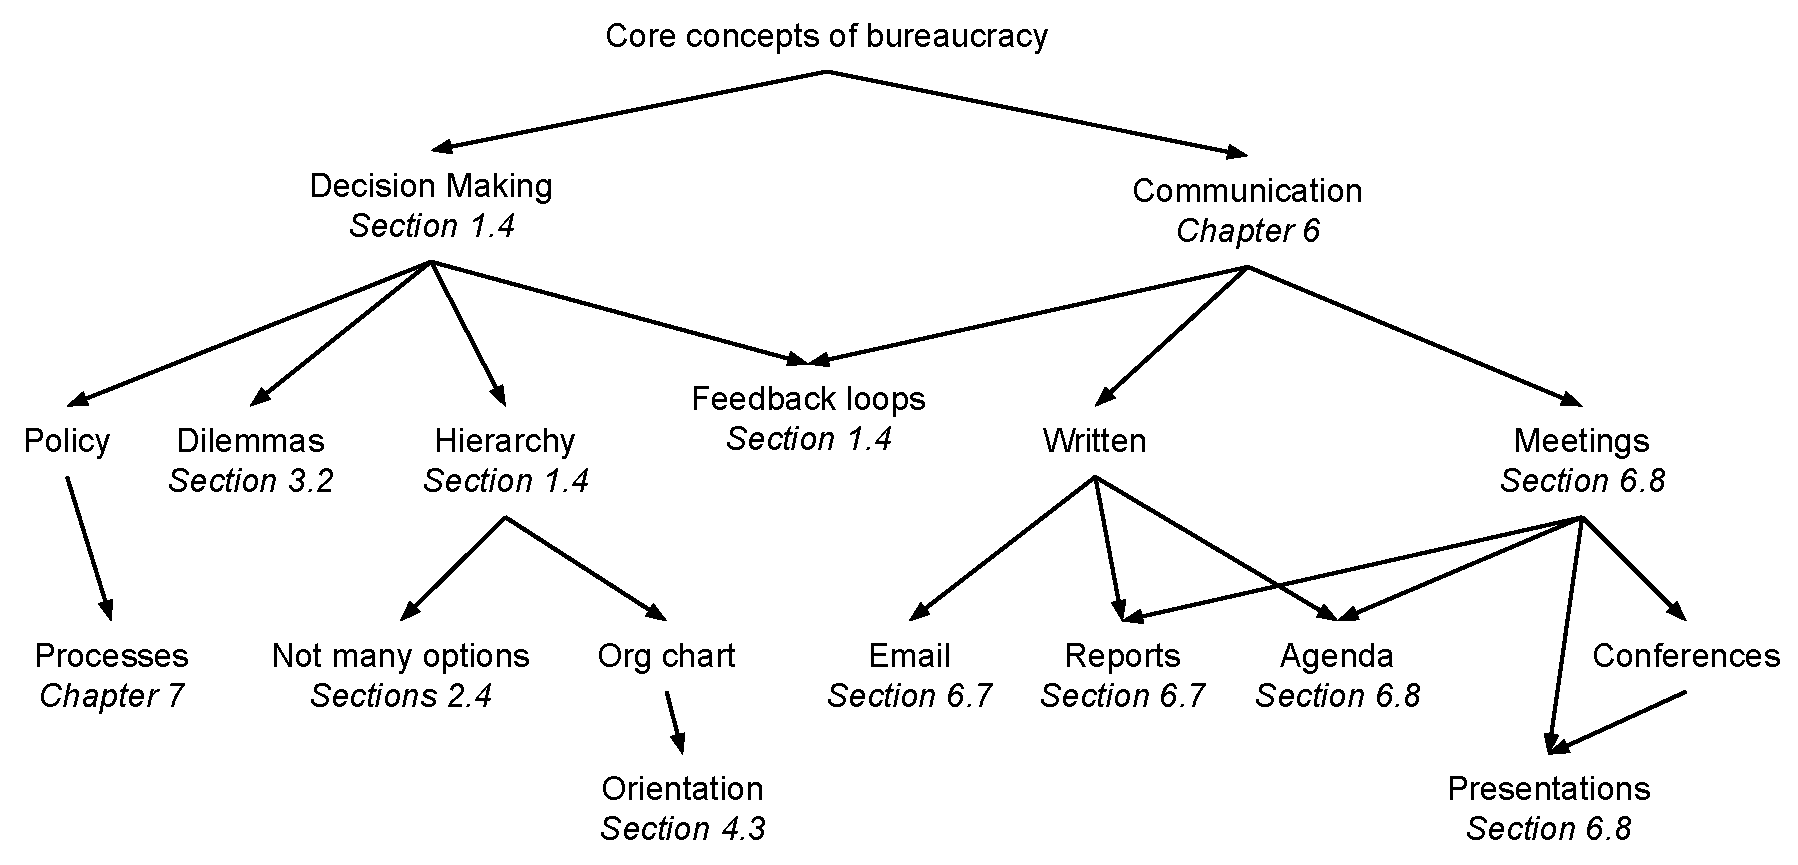
\includegraphics[width=1\textwidth]{images/core_concepts_map.pdf}
    \caption{Relation of the concepts related to bureaucracy discussed in this book. }
    % TODO: include chapter/section in diagram
    % TODO: generate diagram from Latex
    \label{fig:core-concepts}
\end{figure}

% 2022-03-27: BHP was not impressed by the options on https://texample.net//tikz/examples/tag/graphs/ including the "mindmap" option
% this looks better: http://randomresearchdata.blogspot.com/2013/12/tikz-simple-decision-tree-or-cart-tree.html
% see https://texample.net/tikz/examples/feature/trees/

%\begin{tikzpicture}[main/.style = {draw, circle}] 
%\node[main] (1) {Core Concepts}; 
%\node[main] (2) [above right of=1] {Decision Making}; 
%\draw[->] (1) -- (2);
%\end{tikzpicture} 

The approach in this book is to view bureaucracy from a few perspectives. The first is a conceptual view focused on the \hyperref[sec:define-bureaucracy]{definition of bureaucracy} in terms of managing shared resources. The second view is structural (e.g., hierarchy, meetings). The \hyperref[sec:fundamentals-of-b]{essentials of bureaucracy} (starting on page~\pageref{sec:fundamentals-of-b})
will be familiar to experienced bureaucrats. 
The third view is based on experience of the practicing bureaucrat -- \hyperref[sec:dilemma-trilemma]{dilemmas} (page~\pageref{sec:dilemma-trilemma}), \hyperref[sec:unavoidable-hazards]{unavoidable hazards} (page~\pageref{sec:unavoidable-hazards}, and \hyperref[sec:effective-bureaucrat]{tips on how to be effective} (page~\pageref{sec:effective-bureaucrat}). 


%The three productive views of bureaucracy (concept, structure, experience) are contrasted with~\hyperref[sec:alternative-views-from-within]{how other bureaucrats view bureaucracy} and~\hyperref[sec:models-of-bureaucracy]{other models of bureaucracy}.

Chapters~\ref{sec:introduction} to~\ref{sec:why-bur-hard} provide background context for bureaucracy. 
Chapters~\ref{sec:getting-started} to~\ref{sec:process} are the field guide. 
Each chapter capable of being read independently. 



\ \\

% as per https://tex.stackexchange.com/q/393238/235813
\begin{flushright}
Ben Payne\\
\today\\
United States of America\\
Earth
\end{flushright}


